%%%%%%%%%%%%%%%%%%%%%%%%%%%%%%%%%%%%%%%%%%%
	% Capítulo 1
%%%%%%%%%%%%%%%%%%%%%%%%%%%%%%%%%%%%%%%%%%%


\chapter{Aprendizado de Máquina}
\thispagestyle{empty} % retira numeracao da pagina, conforme as normas de apresentacao.
\label{chapter:aprendizadomaquina}

Um dos desafios da Inteligência Artificial é construir sistemas que façam a máquina aprender conceitos e/ou se adaptar ao ambiente. A subárea da Inteligência Artificial relacionada a esse tipo de problema é denominada aprendizado de máquina.\footnote{Neste trabalho, para efeitos de simplificação, quando o termo aprendizado for utilizado, estará se referindo ao aprendizado de máquina} O aprendizado indutivo, um tipo de aprendizado, tem por objetivo inferir padrões ou conhecimento, representados por uma hipótese, ou modelo, a partir de exemplos fornecidos. O aprendizado indutivo pode ser dividido em dois tipos: aprendizado supervisionado e não supervisionado.

No aprendizado supervisionado, cada exemplo fornecido ao indutor possui um rótulo, oferecido por um supervisor especialista do domínio de onde os dados são provenientes. O objetivo do aprendizado supervisionado é construir uma hipótese, ou modelo, que rotule novos exemplos ainda não rotulados. No problema padrão de aprendizado supervisionado, a entrada do algoritmo consiste de um conjunto de objetos rotulados, ou exemplos, $S$, com $N$ objetos $T_i, i=1,...,N$, escolhidos de um domínio $X$ com uma distribuição $\mathcal{D}$ fixa, desconhecida e arbitrária, da forma \{$(\mathbf{x}_i,Y_i),..., \mathbf{x}_N,Y_N)$\} para alguma função desconhecida y = f($\mathbf{x}$). Os $(\mathbf{x}_i$ são tipicamente vetores da forma $(\mathbf{x}_{i1},\mathbf{x}_{i2},...,\mathbf{x}_{iM})$ com valores discretos ou numéricos, e $X_{ij}$ refere-se ao valor do atributo $j$, denominado $X_j$ , do exemplo $T_i$. Os valores $y_i$ referem-se ao valor do atributo $Y$, frequentemente denominado classe. Os valores de $y$ são tipicamente pertencentes a um conjunto discreto de classes $\mathbf{C} = \{\mathbf{C}_1,...,\mathbf{C}_R\}$, quando se trata de classificação, ou ao conjunto de números reais em caso de regressão. Neste trabalho, somente serão abordados problemas de classificação. Assim, quando for dito que um exemplo pertence a uma determinada classe $\mathbf{C}_r$ , isso significa que o exemplo possui $\mathbf{C}_r$ como valor de $y$, ou, ainda, o valor $\mathbf{C}_r$ foi associado a $y$ quando o problema é associar uma classe a um exemplo. O problema de associar somente uma classe a cada exemplo é também denominado aprendizado monorrótulo. No aprendizado não supervisionado, os exemplos não são rotulados, e o objetivo desse aprendizado é realizar descoberta de conhecimento por investigação. Nesse caso, analogamente ao aprendizado supervisionado, o conjunto de objetos não-rotulados $S$ é composto por $N$ objetos $T_i, i=1,...,N$, escolhidos de um domínio $X$ com uma distribuição $\mathcal{D}$ fixa, desconhecida e arbitrária, da forma $\{\mathbf{x}_1,...,\mathbf{x}_N\}$, onde $\mathbf{x}_i$ são tipicamente vetores da forma $(\mathbf{x}_{i1},\mathbf{x}_{i2},...,\mathbf{x}_{iM})$ com valores discretos ou numéricos, e $\mathbf{x}_{ij}$ refere-se ao valor do atributo $j$, denominado $\mathbf{X}_j$ , do exemplo $T_i$. 

\section {Aprendizado de Máquina Não-Supervisionado Hierárquico}

Aprendizado não supervisionado pode ser definido como um modo de encontrar padrões nos dados e ignorar de uma certa maneira o que é considerado puramente ruído. Existem técnicas de aprendizado não supervisionado, como por exemplo, clusterização e redução de dimensionalidade. Ambas consideradas pilares do aprendizado não suupervisionado \cite{conf/ac/Ghahramani03}. 

A técnica de redução de dimensionalidade consiste na redução do número de atributos. O objetivo dessa técnica é obter um conjunto de atributos a partir da redução do espaço de busca pela solução. Portanto o conjunto obtido possui menor dimensionalidade em relação ao conjunto original, entretanto a qualidade da solução final deve ser mantida  \cite{oai:teses.usp.br:tde-06052009-154832}. Embora a técnica de redução de dimensionalidade seja amplamente utilizada, nesse trabalho o nosso enfoque se concentra na técnica de clusterização.

Clusterização, ou análise de cluster, consiste na busca de agrupar elementos de dados baseando-se na similaridade entre eles \cite{Doni:2004}. O objetivo é conseguir determinar os grupos, a fim de obter homogeneidade dentro dos grupos e heterogeneidade entre eles. Devido a grande capacidade de armazenamento de dados, esse grande volume de dados podem gerar muitas combinaçoes de grupos, o que dificulta a sua análise, devido ao grande custo computacional. 

Afim de resolver esse impasse, foram desenvolvidas várias técnicas que auxiliam na formação dos grupos. Algumas caracterısticas são vitais à essas tecnicas, para que
elas consigam um resultado satisfatório, como por exemplo, ser capaz de lidar com dados com alta dimensionalidade, habilidade para lidar com diferentes tipos de dados, entre
outros \cite{conf/pakdd/ZaianeFLW02}. Ainda nessa seção, serão apresentadas técnicas e métricas que auxiliam nessa análise.

Dois fatores são fundamentais no processo de agrupamento: (1) uma medida de similaridade e (2) uma estratégia de agrupamento. A maneira com que os grupos são obtidos está diretamente relacionada a medida de similaridade escolhida, que determinam como a similaridade entre dois elementos é calculada. Essa escolha depende dos tipos de atributos que representam os exemplos \cite{RicardoMarcondes:2014}. Para indução de modelos de agrupamento a partir dos dados, são utilizados métodos e algoritmos, que correspondem às estratégias de agrupamento \cite{hastie2009unsupervised}.


\subsection{Medidas de similaridade}

Medidas de "proximidade" ou "similaridade" são necessárias na maioria das vezes, quando se quer obter de um conjunto de dados complexo, uma estrutura simples de grupos \cite{kasznar2009tecnicas}. Essas medidas são calculadas entre os elementos a serem agrupados. A partir da utilização dessas medidas podem ser definidas as relações intra-cluster, ou seja, as relações definidas, para que elementos pertençam a um mesmo cluster. Normalmente as medidas de similaridade são funções de distâncias ou métricas. Ainda nessa seção, serão apresentadas algumas das medidas de similaridade, expressas por funções de distâncias, comumente utilizadas. 

\subsubsection{Distância Euclidiana}

Distância euclidiana é considera uma distância geométrica no espaço multidimensional. Utilizando dois elementos $X = [X_{1},X_{2}, ... ,X_{p}]$ e $Y = [Y_{1},Y_{2}, ... ,Y_{p}]$ ela pode ser calculada através da equação~\ref{eq:d_euclidiana}:

\begin{equation}\label{eq:d_euclidiana}
	d_{x,y} = \sqrt{(X_{1}-Y_{1})^{^{2}}+(X_{2}-Y_{2})^{^{2}}+...+(X_{p}-Y_{p})^{^{2}}} = \sqrt{\sum_{i=1}^{p}(X_{i}-Y_{i})^{^{2}}} \end{equation}

\subsubsection{Distância Euclidiana Quadrática}

Distância euclidiana quadrática é definida pela equação~\ref{eq:d_euclidiana_quad}:

\begin{equation}\label{eq:d_euclidiana_quad}
	d_{x,y} = (X_{1}-Y_{1})^{^{2}}+(X_{2}-Y_{2})^{^{2}}+...+(X_{p}-Y_{p})^{^{2}} =\sum_{i=1}^{p}(X_{i}-Y_{i})^{^{2}}
\end{equation}

\subsubsection{Distância Manhattan}

Distância Manhattan calcula a distância que seria percorrida para chegar de um ponto de dados para o outro, se um caminho do tipo grade for seguido. A distância Manhattan entre os dois itens é a soma das diferenças dos seus componentes correspondentes, logo pode ser obtida utilizando a equação~\ref{eq:d_manhattan}:

\begin{equation}\label{eq:d_manhattan}
	d_{x,y} = (|X_{1}-Y_{1}|)+(|X_{2}-Y_{2}|)+...+(|X_{p}-Y_{p}|) =\sum_{i=1}^{p}(|X_{i}-Y_{i}|)
\end{equation}

\subsubsection{Distância Chebychev}

Distância Chebychev é utilizada, na situação que se deseja diferenciar dois elementos, se houver apenas uma das dimensões diferente, a distância de chebychev é definida pela equação~\ref{eq:d_chebychev}:

\begin{equation}\label{eq:d_chebychev}
	d_{x,y} = max(|X_{1}-Y_{1}|)+(|X_{2}-Y_{2}|)+...+(|X_{p}-Y_{p}|)
\end{equation}

\subsection{Métodos de Agrupamento}

Métodos de agrupamento podem ser organizados em dois tipos \cite{rokach2009survey}: agrupamento particional e agrupamento hierárquico. No primeiro tipo, um conjunto de exemplos é dividido em uma partição simples de $k$ grupos. Enquanto no segundo, exemplos são organizados em grupos e subgrupos a partir de uma sequência de partições aninhadas \cite{RicardoMarcondes:2014}. 

O método proposto nesse trabalho utiliza a abordagem de clusterização hierárquica, portanto, a seguir iremos apresentar com mais detalhes alguns métodos hierárquicos utilizados para realizar agrupamentos.

\subsubsection{Métodos hierárquicos}

Os métodos hierárquicos de clusterização consistem em uma série de sucessivos agrupamentos (clusters) ou sucessivas divisões de elementos, onde esses elementos são agregados ou desagregados \cite{Doni:2004}. A distância entre os clusters é usada como critério para formação dos mesmos \cite{carvalho2009clusterizaccao}. Pode acontecer de um exemplo pertencer a mais de um grupo, ou até mesmo, ocorrer de cada exempo possuir um grau de pertinência associado aos grupo. A ocorrência de alguma dessas situações é chamada de sobreposição \cite{RicardoMarcondes:2014}. 

%Os métodos hierárquicos são divididos em métodos aglomerativos e métodos divisivos, essas abordagens serão apresentadas a seguir.

A clusterização hierárquica pode ser feita de duas formas: aglomerativa – iniciando com tantos clusters quantos objetos e então unindo-os em novos clusters – ou divisiva – iniciando com um cluster apenas e dividindo-o em novos clusters \cite{carvalho2009clusterizaccao}. As duas abordagens são apresentadas a seguir.

\subsubsection{Métodos aglomerativos}

Os dados são inicialmente distribuídos de modo que cada exemplo represente um cluster e, então, esses clusters são recursivamente agrupados considerando alguma medida de similaridade, até que todos os exemplos pertençam a apenas um cluster \cite{berkhin2006survey}, representa uma estratégia \textit{bottom-up} de agrupamento. Existem vários métodos aglomerativos, a característica utilizada para classificar esses métodos é o critério utilizado para definir as distâncias entre grupos, ou seja, as distâncias inter-cluster \cite{Doni:2004}. 

[colocar figura de clusters do método aglomerativo]

Em geral, os métodos aglomerativos utilizam os passos de um algoritmo padrão. A diferença entre os métodos ocorre no passo, onde a função de distância é definida. Os passos do algoritmo padrão e os métodos aglomerativos são apresentados a seguir.

% \begin{figure}[!htb]
%    \centering
%    \includegraphics[scale=0.5]{algpadrao}
%    \caption{Algoritmo Padrão}
%  \end{figure}

\IncMargin{1em}
\begin{algorithm}[H]
\SetAlgoLined
\SetKwInOut{Input}{Entrada}\SetKwInOut{Output}{Saída}
\SetKwRepeat{Do}{do}{while}
\Input{Base de dados com \textbf{N} elementos}
\Output{Um conjunto de grupos }
Iniciar com \textbf{N} grupos, cada grupo contendo um elemento e uma matriz de similaridade $\mathbf{D_{nXn}}$\\
\Repeat{\textbf{N-1, no qual todos elementos estarão em um único grupo}}{
Encontrar a menor distância $\mathbf{d_{uv}}$ (maior similaridade)\;
Atualizar a matriz \textbf{D}, removendo os elementos \textbf{U} e \textbf{V}\;
Atualizar a matriz \textbf{D}, inserindo as novas distâncias do grupo \textbf{(U,V)}\;
}
\caption{Algoritmo padrão utilizado por métodos aglomerativos.}
\end{algorithm}
\DecMargin{2em}

\paragraph{Simple Linkage:} 

Conhecido também como, método de ligação por vizinho mais próximo, esse método utiliza a distância de menor valor, distância definida pela expressão ~\ref{eq:simple_lkg}: 

\begin{equation}\label{eq:simple_lkg}
d_{(UV)W} = min(d_{UW},d_{VW})
\end{equation}

Segundo \cite{anderberg1973}, são essas algumas características desse método: Geralmente, grupos muito próximos podem não ser identificados; Possibilita a detecção de grupos que possuem formas não-elípticas; Apresenta pouca tolerância a ruído; Demonstram bons resultados utilizando distâncias euclidianas assim como outras distâncias; Possui a tendência de formar longas cadeias (encadeamento).

\paragraph{Complete Linkage:}

Conhecido também como, método de ligação do vizinho mais distante, esse método utiliza a distância máxima, que é dada pela expressão~\ref{eq:complete_lkg}:

\begin{equation}\label{eq:complete_lkg}
d_{(UV)W} = max(d_{UW},d_{VW})
\end{equation}

Segundo \cite{kaufman1990finding}, são essas algumas características desse método: Demonstra bons resultados utilizando distâncias euclidianas assim como outras distâncias; Possui a tendência de formas grupos compactos; Os ruídos demoram a serem inseridos ao grupo.

\paragraph{Average Linkage:}

Conhecido também como, método de ligação por média, esse método utiliza a expressão ~\ref{eq:average_lkg}, para o cálculo da distância:

\begin{equation}\label{eq:average_lkg}
d_{(UV)W} = \frac{(N_{U}.d_{UW} + N_{V}.d_{VW})}{N_{U}+N_{V}}
\end{equation}

- onde $N_{U}$ e $N_{V}$ são os números de elementos no grupo U e V, respectivamente; $d_{UW}$ e $d_{VW}$ são as distâncias entre os elementos UW e VW, respectivamente.  

Segundo \cite{kaufman1990finding}, são essas algumas características desse método: Menor sensibilidade à ruídos comparado aos métodos de ligação por vizinho mais próximo e vizinho mais distante; Demonstra bons resultados utilizando distâncias euclidianas assim como outras distâncias; Possui a tendência de formar grupos com número de elementos similares

\paragraph{Centroid Linkage:}

Conhecido também como, método de ligação por centróide, esse método utiliza a expressão~\ref{eq:centroid_lkg}, para o cálculo da distância:

\begin{equation}\label{eq:centroid_lkg}
d_{(UV)W} = \frac{(N_{U}.d_{UW} + N_{V}.d_{VW})}{N_{U}+N_{V}} - \frac{N_{U}.N_{V}.d_{UW}}{(N_{U} + N_{V})^{^{2}}}
\end{equation}

- onde $N_{U}$ e $N_{V}$ são os números de elementos no grupo U e V, respectivamente; $d_{UW}$ e $d_{VW}$ são as distâncias entre os elementos UW e VW, respectivamente. 

\paragraph{}
Segundo \cite{Doni:2004}, são essas algumas características desse método: Robustez à presença de ruídos; Passível de ocorrência do fenômeno da reversão, isto ocorre quando a distância entre os centróides é menor que a distância entre grupos já formados, consequentemente fará com que os novos grupos se formem ao um nível inferior aos grupos existentes. Esse método não é muito utilizado, pois devido a ocorrência do fenômeno da reversão, o resultado é um dendograma confuso.

\paragraph{Median Linkage:}

Conhecido também como, método de ligação por mediana, esse método utiliza a seguinte expressão, para o cálculo da distância:

\begin{equation}\label{eq:median_lkg}
d_{(UV)W} = \frac{d_{UV} + d_{VW}}{2} - \frac{d_{UV}}{4}
\end{equation}

- onde  $d_{UW}$ e $d_{WV}$ são as distâncias entre os elementos UW e VW, respectivamente. 

\paragraph{}
Segundo \cite{Doni:2004}, são essas algumas características desse método: Demonstra resultados satisfatórios quando os grupos são de tamanhos diferentes; Quando permutado os elementos na matriz de similaridade, pode apresentar resultado diferente; Robustez á presença de \textit{outliers}.

\paragraph{Ward's Linkage:}

Método de ligação de Ward, nesse método a distância é calculada pea expressão:

\begin{equation}\label{eq:ward_lkg}
d_{(UV)W} = \frac{((N_{W}+N_{U}).d_{UW} + (N_{W}+N_{V}).d_{VW} - N_{W}.d_{UV})}{N_{W}+N_{U}+N_{V}}
\end{equation}

- onde $N_{U}$ e $N_{W}$ são os números de elementos no grupo U e V, respectivamente; $d_{UW}$ e $d_{VW}$ são as distâncias entre os elementos UW e VW, respectivamente.

\paragraph{}
Segundo \cite{Doni:2004}, são essas algumas características desse método: Demonstra bons resultados utilizando distâncias euclidianas assim como outras distâncias; Se o número de elementos em cada grupo for praticamente igual, o método pode apresentar resultados insatisfatórios; Possui a tendência de combinar grupos com poucos elementos; Sensível à presença de \textit{outliers}.

\subsubsection{Métodos divisivos}

O processo inicia-se com apenas um agrupamento contendo todos os dados e segue dividindo-o recursivamente segunda alguma métrica até que alcance algum criterio de parada, frequentemente o número de clusters desejados \cite{berkhin2004survey}. 

[colocar figura de clusters do método aglomerativo]

Devido a exigência de maior capacidade computacional, os métodos divisivos são pouco citados na literatura em relação aos métodos aglomerativos  \cite{kaufman1990finding}. A seguir será apresentado o método divisivo proposto por \cite{macnaughton1964dissimilarity}. 

\paragraph{MACNAUGHTON-SMITH:}

O custo computacional demandado por métodos divisivos é alto. O que pode tornar a implementação inviável, caso o número de elementos seja grande e conjunto de divisões possíveis for todo considerado, o número de iterações pode aumentar exponencialmente. Entretanto o método proposto por MacNaughton-Smith, é capaz de evitar esse problema \cite{Doni:2004}. O pseudo-código do algoritmo de MacNaughton-Smith será apresentado abaixo.



%Consegue contornar o problema de crescimento exponencial de iterações, que ocorre quando o número de  que é o responsável por tornar a implementação inviável, quando considerado todo o conjunto de divisões possíveis. A figura 3, apresenta a descrição do algoritmo utilizado nesse método.%

%\begin{figure}[!htb]
%   \centering
%   \includegraphics[scale=0.5]{mc}
%   \caption{MacNaughto... pseudo codigo}
%\end{figure}

\IncMargin{1em}
\begin{algorithm}[H]
\SetAlgoLined
\SetKwInOut{Input}{Entrada}\SetKwInOut{Output}{Saída}
\SetKwRepeat{Do}{do}{while}
\Input{Base de dados com \textbf{N} elementos}
\Output{Um conjunto de grupos }
\textbf{j=1}\\
\Repeat{restarem apenas grupos com dois elementos}{
	Selecionar o grupo $\mathbf{G_j}$ com maior número de elementos $\mathbf{N_j}$\;
    Iniciar uma matriz $\mathbf{D_{nj}xD_{nj}}$\;
    Calcular a similaridade média $\mathbf{S_m}$ de cada elemento do grupo $\mathbf{G_j}$ em relação aos demais\;
    \While{$\mathbf{S_m} > 0$}{
       Remover o elemento $\mathbf{e}$ com maior $\mathbf{S_m}$ do grupo $\mathbf{G_j}$\;
       Armazenar o elemento $\mathbf{e}$ no grupo $\mathbf{F_j}$\;
       (re)Calcular a similaridade média $\mathbf{S_i}$ entre os elementos que restaram no grupo $\mathbf{G_j}$\;
       (re)Calcular a similaridade média $\mathbf{S_a}$ entre cada elemento do grupo $\mathbf{G_j}$ e o grupo $\mathbf{F_j}$\;
       $\mathbf{S_m = S_i - S_a}$\;
    }
	\textbf{j=j+1}\\   
}
\Repeat{que todos grupos sejam divididos}{
  Selecionar o grupo \textbf{H} com maior similaridade média\;
  Dividir o grupo \textbf{H}\;
}
\caption{Pseudo-código do algoritmo divisivo de MACNAUGHTON-SMITH}
\end{algorithm}
\DecMargin{2em}
\newpage
\section {Aprendizado de Máquina Multirrótulo}

Tanto o aprendizado de máquina supervisionado quanto o não supervisionado podem ser aplicados nas mais diversas áreas de conhecimento, e nos mais diversos tipos de problemas existentes no mundo real. Como problemas do mundo real, podemos citar a simulação de situações de emergência, jogos, biomedicina, dentre outros \cite{faceli2011inteligencia}. Entretanto, dentre essas áreas de aplicação, há problemas nos quais mais de um rótulo são associados aos exemplos utilizados como treinamento. Exemplos desse tipo de problema são associação de rótulos a imagens (uma imagem pode ter associado vários nomes indicando diferentes objetos na imagem) \cite{shen2004multilabel}, associação de palavras-chaves a documentos textuais \cite{sebastiani2002machine,schapire2000boostexter}, associação de anotações a vídeos \cite{dimou2009empirical}, associação de gêneros musicais a músicas \cite{lukashevich2009multi}, predição de falhas a equipamentos \cite{bernardini2009artificial}, dentre outros. Para esse tipo de problema, pode ser interessante induzir um classificador que rotule novos exemplos com mais de um rótulo. Para induzir modelos com essa característica, deve ser utilizado o aprendizado de máquina multirrótulo. Para um algoritmo de aprendizado de um modelo multirrótulo, a entrada consiste de um conjunto de exemplos $S$, com $N$ objetos rotulados, ou exemplos, $T_i, i=1,...,N$, escolhidos de um domínio $X$ com uma distribuição $\mathcal{D}$ fixa, desconhecida e arbitrária, da forma \{$(\mathbf{x}_i,Y_i),..., \mathbf{x}_N,Y_N)$\}. $L$ é o conjunto de rótulos possíveis do domínio $D$, e $Y_i \subseteq L$, ou seja, $Y_i$ é o conjunto de rótulos associado ao i-ésimo objeto. A saída de um algoritmo de aprendizado supervisionado de modelos multirrótulos é um classificador \textbf{h}, que classifica um exemplo $\mathbf{x_i}$ com o conjunto $\mathbf{Z_i = h(x_i)}$, o qual é o conjunto de classes preditas por $\mathbf{h\{x\}}$ para o exemplo $\mathbf{x_i}$ . Há diversos métodos propostos na literatura para indução de modelos multirrótulo \cite{tsoumakas2010mining,calembo2011proposta,alvares2012incorporating,da2013rb}.


%No aprendizado supervisionado, cada exemplo fornecido ao indutor possui um rótulo, oferecido por um supervisor especialista do domínio de onde os dados são provenientes. O objetivo do aprendizado supervisionado é construir uma hipótese, ou modelo, que rotule novos exemplos ainda não rotulados. No problema padrão de aprendizado supervisionado, a entrada do algoritmo consiste de um conjunto de objetos rotulados, ou exemplos, $S$. O problema de associar somente uma classe a cada exemplo é também denominado aprendizado monorrótulo. No aprendizado não supervisionado, os exemplos não são rotulados, e o objetivo desse aprendizado é realizar descoberta de conhecimento por investigação. Como problemas do mundo real, podemos citar a simulação de situações de emergência, jogos, biomedicina, dentre outros \cite{faceli2011inteligencia}. Entretanto, dentre essas áreas de aplicação, há problemas nos quais mais de um rótulo são associados aos exemplos utilizados como treinamento. Exemplos desse tipo de problema são associação de rótulos a imagens (uma imagem pode ter associado vários nomes indicando diferentes objetos na imagem), associação de palavras-chaves a documentos textuais, associação de anotações a vídeos, associação de gêneros musicais a músicas, predição de falhas a equipamentos, dentre outros. Para esse tipo de problema, deve ser utilizado o aprendizado multirrótulo, cuja entrada consiste de um conjunto de exemplos rotulados $S$, e cuja saída é um classificador multirrótulo. Há diversos métodos propostos na literatura para indução de modelos multirrótulo \cite{tsoumakas2010mining}. É importante avaliar a complexidade de conjuntos de dados multirrótulo. A cardinalidade de um conjunto de dados multirrótulo é dada pelo número médio de rótulos dos exemplos, e é independente do número de possíveis rótulos. Já a densidade de um conjunto de dados multirrótulo é dada pelo número médio de rótulos dos exemplos dividido pelo número total de rótulos. 


\section {Métodos de Aprendizado Multirrótulo}

Existem duas categorias principais que podemos agrupar os métodos de aprendizado multirrótulo \cite{tsoumakas2007multi}. Apesar de serem métodos multirrótulo, a regra para realizar essa categorização está associada ao modo que algoritmos de classificação monorrótulo são utilizados \cite{tsoumakas2009mining}.

A primeira categoria é chamada de \textit{Transformação de Problema}. O próprio nome é intuitivo e sugestivo, nessa categoria, problemas de classificação multirrótulo são transformados em um ou mais problemas de classificação monorrótulo \cite{chermanaprendizado}. A partir dessa transformação, o processo de classificação é executado da mesma maneira que em problemas de classificação monorrótulo \cite{modi2012experimental}. Isto é, para cada problema monorrótulo transformado, são utilizados algoritmos de classificação monorrótulo para resolvê-los \cite{chermanaprendizado}. Métodos pertencentes a categoria de transformação de problema também são chamados de métodos independente de algoritmo \cite{modi2012experimental}.
Já a segunda categoria, \textit{Adaptação de algoritmo}, nenhuma transformação é realizada \cite{chermanaprendizado}. Portanto, o problema multirrótulo é tratado diretamente, através de modificações em algoritmos existentes\cite{modi2012experimental}. Essa abordagem de criação de métodos específicos para tratar problemas multirrótulo é chamada de abordagem dependente de algoritmo \cite{faceli2011inteligencia}. 

A seguir serão apresentados alguns exemplos de métodos pertencentes às ambas categorias.

\subsection{Métodos de Transformação de Problema}

Métodos de transformação de problema se utilizam da abordagem independente de algoritmo. Portanto, para resolver o problema pode ser utilizado qualquer algoritmo tradicional. O processo  para resolução do problema é feito através da realizacão da transformacão do problema multirrótulo original em um conjunto de problemas de classificação monorrótulo. Essa transformação pode ser baseada em dois tipos\cite{faceli2011inteligencia}:
\newline
\newline
 1 - Baseada nos Rotulos das Classes;
\newline
 2 - Baseada nos Exemplos; 
 
\paragraph{}
No tipo de transformação baseada nos rótulos das classes, tomando um problema onde $k$ é o numero de classes, e $k$ classificadores são utilizados. Cada classificador é associado a uma classe e treinado para resolver um problema de classifição binária \cite{faceli2011inteligencia}. Um popular método de transformação de problemas baseado nos rótulos das classes é o \textit{Binary Relevance}(BR)\cite{tsoumakas2009mining}. Por outro lado, no segundo tipo de transformação, o resultado do método não é somente problemas de classificão binária, mas também pode ser produzido problemas multiclasse. Porquanto na transformação baseada nos exemplos, o conjunto de classes associado a cada exemplo é redefinido \cite{faceli2011inteligencia}. Um exemplo de método desse tipo amplamente utilizado é o \textit{Label Powerset} (LP)\cite{tsoumakas2009mining}.
 
A tabela ~\ref{tab:conjunto_multirrotulo_br_lp} apresenta um exemplo de conjunto de dados multirrótulo, que serve como base para exibir um exemplo de execução dos métodos BR e LP.

%  \begin{figure}[!htb]\
%    \centering
%    \includegraphics[scale=0.5]{exDataSetBRLP}
%    \caption{Exemplo conjunto de dados para exemplo BR e LP}
%  \end{figure}

\begin{table}[h!]
    \centering
   \label{tab:conjunto_multirrotulo_br_lp}
    \begin{scriptsize}
       \begin{tabular}{c|c}

\hline
  	    &       Y	    			\\	\hline\hline
$X_1$	&	$Y_1 = \{y_2,y_3\}$	\\	\hline
$X_2$	&	$Y_2 = \{y_1,y_3,y_4\}$		\\	\hline
$X_3$	&	$Y_3 = \{y_4\}$		\\	\hline
$X_4$	&	$Y_4 = \{y_2,y_3\}$		\\	\hline

\end{tabular}
   \end{scriptsize}
\caption{Exemplo de conjunto de dados multirrótulo}
%\end{minipage}
\end{table}

O \textbf{Binary Relevance (BR)} é um popular método de transformação de problema, que decompõe um problema de classificação multirrótulo em vários diferentes problemas de classificação binária monorrótulo, um para cada $q$ rótulos diferente no conjunto original $S$ \cite{cherman2011multi}. Por conseguinte são aprendidos pelo BR $q$ classificadores binários. O método BR transforma o conjunto de dados $S$ em $|L|$ conjunto de dados $S_j,j=1,...,|L|$ que contém todos os exemplos do conjunto de dados original, rotulados positivamente se o conjunto de rótulos do exemplo original continha o rótulo $j$ e negativamente caso contrário \cite{tsoumakas2011random}. 

A tabela TX apresenta o processo de transformação realizado pelo método BR em quatro conjunto de dados monorrotulo. 

[fazer tabela nativo do latex]

 \begin{figure}[!htb]
    \centering
    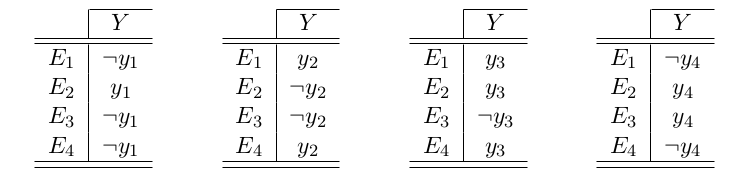
\includegraphics[scale=0.5]{figures/exemploBR}
    \caption{Tabelas monorrótulo resultantes da aplicação do método BR no conjunto multirrótulo ilustrado na Tabela 2.2}
  \end{figure}

Para classificação de uma nova instância, BR dá como saída a união dos rótulos $\lambda$, que são positivamente preditos pelos $q$ classificadores \cite{tsoumakas2011random}.
O Binary Relevance é muito utilizado e apresenta resutados satisfatórios para diversos problemas, entretanto, sua limitação é nao levar em conta as informações de relacionamento entre rótulos, isto é, a dependência de rótulos \cite{chermanaprendizado}. 

\paragraph{}
Já o \textbf{Label Powerset (LP)}, transforma um problema multirrótulo em um problema de classificação multiclasse monorrótulo, onde os possíveis valores para atributos da classe de transformação são o conjunto de únicos e distintos subconjuntos de rótulos
presentes no conjunto de treino original. A aprendizagem a partir de exemplos multirrótulo correspondem em encontrar um mapeamento a partir do espaço de características dos conjuntos de rótulos, ou seja, o poder dos conjuntos de todos os rótulos.

A tabela ~\ref{tab:conjunto_monorrotulo_multiclasse_lp} apresenta o resultado da execução do método LP tornando um conjunto de dados multirrótulo num monorrótulo multiclasse.

% \begin{figure}[!htb]
%    \centering
%    \includegraphics[scale=0.5]{exLP}
%    \caption{Tabelas monorrótulo multiclasse resultantes da aplicação do método LP no conjunto multirrótulo ilustrado na Tabela 2.2}
%  \end{figure}
  
\begin{table}[h]
\label{tab:conjunto_monorrotulo_multiclasse_lp}
\centering
    \begin{scriptsize}
       \begin{tabular}{c|c}

\hline
  	    &       Y	    			\\	\hline\hline
$X_1$	&	$y_{2,3}$	\\	\hline
$X_2$	&	$y_{1,3,4}$		\\	\hline
$X_3$	&	$y_4$		\\	\hline
$X_4$	&	$y_{2,3}$		\\	\hline

\end{tabular}
   \end{scriptsize}
%\end{minipage}
\caption{Conjunto monorrótulo multiclasse resultante da aplicação do método LP no conjunto multirrótulo ilustrado na Tabela ~\ref{tab:conjunto_multirrotulo_br_lp}}
\end{table}

Dado um novo exemplo, o classificador monorrótulo do LP dá como saída a classe mais provável, que é um conjunto de rótulos \cite{modi2012experimental}. Logo, a determinação da classe mais provável é dado de acordo com o valor de predição obtido através de um algoritmo multiclasse treinado com um conjunto de exemplos que foi gerado a partir da transfomação do problema \cite{chermanaprendizado}. Diferentemente do metodo BR o método Label Powerset leva em consideração a dependência de rótulos \cite{modi2012experimental}. Uma limitação do LP se dá ao aumento exponencial do número de possíveis conjuntos de dados, por consequência de considerar dependências dos rótulos durante a classificação, quando uma quantidade grande ou moderada de rótulos são considerados. LP pode ter sua performance comprometida caso existirem classes no conjunto de treino que representem muito poucos exemplos. Quando isso de fato ocorre, é conhecido como problema de desbalanciamento de classe \cite{cherman2011multi}.

\subsection{Métodos de Adaptação de Algoritmo}

Métodos de adaptação de algoritmo se utilizam da abordagem dependente de algoritmo. Logo, com o intuito de tratar os problemas de classificação multirrótulo diretamente, como um todo, novos algoritmos são propostos. Por se tratar de um algoritmo específico, pode apresentar resultados melhores do que métodos que seguem abordagem independente de algoritmo para um determinado problema de classificação real \cite{faceli2011inteligencia}. Um exemplo de método de adaptação de algoritmo proposto é o \textbf{Hierarchy Of Multi-label classifERs (HOMER)} \cite{tsoumakas2008effective}.

O HOMER utiliza a técnica de projeto de algoritmos, dividir e conquistar, com isso, HOMER constrói uma  hierarquia de classificadores multirrótulo, onde cada um lida com um conjunto de rótulos muito menor comparado com o conjunto total de rótulos, por conseguinte, um maior balanceamento na distribuição dos exemplos \cite{tsoumakas2008effective}. Na figura ~\ref{fig:hierarquia_homer} é apresentado um exemplo simples da hierarquia constrída pelo HOMER para uma tarefa de classificação multirrótulo com 8 rótulos. 

  \begin{figure}[!htb]
    \centering
    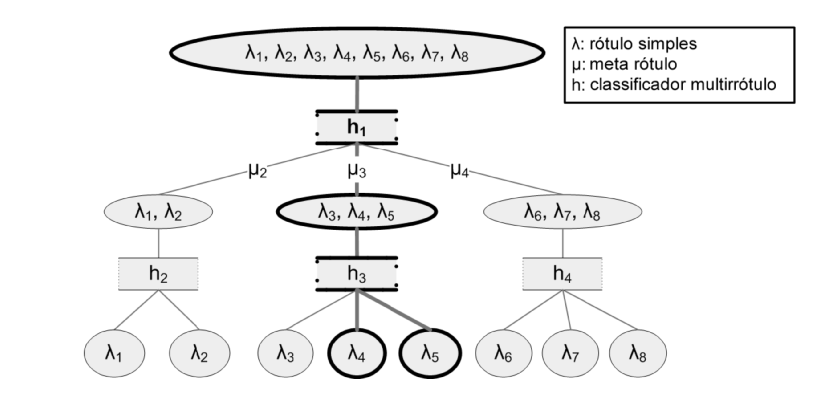
\includegraphics[scale=0.5]{figures/HOMERHierarquia}
    \caption{Hierarquia de rotulos e classificadores construida pelo HOMER  \cite{tsoumakas2008effective}}
    \label{fig:hierarquia_homer}
  \end{figure}

Um dos principais processos internos do HOMER é a distribuição uniforme de um conjunto de rótulos em subconjuntos disjuntos $k$ de modo que os rótulos semelhantes são colocados juntos e os rótulos que não possuem nenhuma semalhança são colocados aparte. Para execução dessa tarefa o HOMER utiliza um algoritmo chamado de \textit{balanced k-Means} \cite{tsoumakas2008effective}. O algoritmo \textit{balanced k-Means} é uma extensao do algoritmo \textit{k-Means} \cite{macqueen1967some}, logo o que difere os dois algoritmos é a utlizacao de uma constante explícita referente ao tamanho de cada cluster e a limitação do número de iterações usando um parâmetro especificado pelo usuário. A peça chave desse algoritmo é que para cada cluster $i$ é mantido uma lista de rotulos, $C_i$, ordenada em ordem ascendente da distancia dos rótulos para o centroid do cluster $c_i$. Quando uma inserção de um rótulo na lista ordenada de cluster feita na posição correta, ocasionar em um estouro do tamanho máximo de rótulos permitidos, na lista de rótulos desse cluster, é selecionado o último rótulo, no caso o mais distante. Esse rótulo selecionado é inserido na lista do próximo cluster mais próximo.  Isto pode levar a $k - 1$  inserções adicionais em cascata no pior caso \cite{tsoumakas2008effective}. O pseudo-código do algoritmo \textit{balanced k-Means} é apresentado a seguir.\\

%\begin{figure}[!htb]
%    \centering
%    \includegraphics[scale=0.5]{Balancedkmenas}
%    \caption{Substituir pelo algoritmo traduzido}
%  \end{figure}

\IncMargin{1em}
\begin{algorithm}[H]
\SetAlgoLined
\SetKwInOut{Input}{Entrada}\SetKwInOut{Output}{Saída}
\Input{número de cluster $k$, rótulos $L_n$, dados de rótulos $W_i$, iterações $it$}
\Output{$k$ clusters balanceados de rótulos }
\For{$i\leftarrow 1$ \KwTo $k$}{
  //inicializa clusters e seus centros\;
  $C_i \leftarrow 0$\;
  $c_i \leftarrow$ membro aleatório de $L_n$\;
}
\While{{$it$ > 0}}{
	\For{\textbf{each} $\lambda \in L_n$}{
    	\For{$i\leftarrow 1$ \KwTo $k$}{
          $d_{\lambda i} \leftarrow distancia(\lambda,c_i,W_i)$\;
        }
        finalizado $\leftarrow$ false\;
        $v \leftarrow \lambda$\;
        \While{{\textbf{not} finalizado}}{
           $j \leftarrow $ arg min $d_{vi}$\;
           Insere $ordena (v,d_v)$ na lista ordenada $C_j$\;
           \eIf{$|C_j| > [|L_n|/k]$}{
      			$v \leftarrow$ remove último elemento de $C_j$\;
      			$d_{vj} \leftarrow \infty$\;
    	   }{
     			 finalizado $\leftarrow$ true\;
   		   }
        }
    }
    recalcula centros\;
    $it \leftarrow it -1$\;
}
\Return $C_1,...,C_k$\;
\caption{Algoritmo Balanced k-Means}
\end{algorithm}
\DecMargin{1em}

%Figura X1 - Algoritmo Balanced k means.
\newpage

O método HOMER foi construído para lidar com problemas de classifição multirrótulo com domínios que possuam muitos rótulos de maneira efetiva e computacionalmente eficiente. A partir dessa estratégia de hierarquia de classificadores, o HOMER melhora a predição com complexidade linear para treinamento, e logarítma para teste no que se refere a quantidade total de rótulos \cite{tsoumakas2008effective}.


\section {Características de Conjuntos de Dados Multirrótulo}

Os conjuntos de dados não são todos igualmente multirrótulo. Em alguns casos, o número de classes de cada exemplo é pequeno se comparado ao número total de exemplos $n$, enquanto em outros, esse número é grande. Esse número pode ser parâmetro que influencia o desempenho dos diferentes métodos de classificação multirrótulo. Existem duas medidas para avaliar as características de um conjunto de dados: cardinalidade $Card(S)$ e densidade $Dens(S)$ \cite{tsoumakas2010mining}.

A cardinalidade de um conjunto de dados multirrótulo $S$ – $Card(S)$ – é dada pelo número médio de rótulos dos exemplos $T_i \in S$, e é independente do número de possíveis rótulos $|L|$ – Equação  ~\ref{eq:Cardinalidade}. Essa medida é utilizada para quantificar o número de rótulos alternativos que caracterizam os exemplos de um conjunto de dados multirrótulo.
        
A densidade de um conjunto de dados multirrótulo $S$ – $Dens(S)$ – é dada pelo número médio de rótulos dos exemplos que pertencem a $S$ dividido pelo número total de rótulos $|L|$ – Equação \ref{eq:Densidade}. A densidade de rótulo leva o número de possíveis rótulos em consideração.

\begin{equation}\label{eq:Cardinalidade}
    Card(S) = \frac{1}{N}\sum_{i=1}^{N}{|Y_i|}
\end{equation}

\begin{equation}\label{eq:Densidade}
    Dens(S) = \frac{1}{N}\sum_{i=1}^{N}{\frac{|Y_i|}{|L|}}
\end{equation}

\section {Avaliação de Algoritmos de Aprendizado Multirrótulo}

Para avaliar os classificadores multirrótulo, existem três grupos de medidas para avaliação induzida:
baseada em instâncias, baseadas em rótulos e baseadas em ranking \cite{dimou2009empirical}. Neste trabalho, somente são usados os primeiros dois grupos de medidas, pois ranking multirrótulo não é o foco desse trabalho. Do primero grupo, são usadas nesse trabalho \textit{Hamming Loss} ($Ham$), \textit{Subset Accuracy} ($SA$) e $F$, definidas pelas equações~\ref{hammingLoss} à~\ref{f-measure}\footnote{Na Eq.~\ref{hammingLoss}, $\Delta$ representa a difereça simétrica entre dois conjuntos.}, respectivamente. Do segundo grupo, são usados as versões micro e macro da medida $F1$. Medidas baseada em rótulos são calculadas baseadas em falso positivos $f_p$, falso negativos $f_n$, verdadeiro positivos $t_p$ e verdadeiro negativos $t_n$, \textit{i.e.}, medidas do tipo $B(t_p, t_n, f_p, f_n)$ podem ser usadas nesse caso. Dado que $t_{p_l}$, $t_{n_l}$, $f_{p_l}$ e $f_{n_l}$ são verdadero positivos, verdadeiro negativos, falso positivos e falso negativos para cada rótulo $l \in L$, a versão micro das medidas $B$ é denotada por $B_{-}$ é dada pela Eq.~\ref{eq:micro}, enquanto que a versão macro das medidas $B$ é denotada por $B^{-}$ é dada pela Eq.~\ref{eq:macro}. In this work, we only use $F1$ as a $B$ measure, and $F1(t_p, t_n, f_p, f_n)$ is given by Eq.~\ref{eq:F1}.

\begin{equation}\label{hammingLoss}
    Ham(\mathbf{h},S) = \frac{1}{N}\sum_{i=1}^{N}\frac{|Y_i\Delta Z_i|}{|L|}
\end{equation}

\begin{equation}\label{subAcc}
    SA(\mathbf{h},S) = \frac{1}{N}\sum_{i=1}^{N}I(Z_i = Y_i)
\end{equation}

\begin{equation}\label{f-measure}
    F(\mathbf{h},S) = \frac{1}{N}\sum_{i=1}^{N}\frac{2|Y_i \cap Z_i|}{|Z_i| + |Y_i|}
\end{equation}

\begin{equation}\label{eq:micro}
%    \begin{split}
    B_{-}(\mathbf{h},S) = \frac{1}{|L|}\sum_{i=1}^{|L|}B(t_{p_i},t_{n_i},f_{p_i},f_{n_i})
%    \end{split}
\end{equation}

\begin{equation}\label{eq:macro}
%    \begin{split}
     B^{-}(\mathbf{h},S) = \frac{1}{|L|}B(\sum_{i=1}^{|L|}t_{p_i},\sum_{i=1}^{|L|}t_{n_i},\sum_{i=1}^{|L|}f_{p_i},\sum_{i=1}^{|L|}f_{n_i})
%    \end{split}
\end{equation}

\begin{equation}\label{eq:F1}
%    \begin{split}
      F1(t_p, t_n, f_p, f_n) = \frac{2 \times f_p}{2 \times t_p + f_n + f_p}
%    \end{split}
\end{equation}
